\documentclass{scrreprt}

\usepackage{graphicx}
\usepackage[a4paper,top=1in,bottom=1in,right=0.6in,left=0.6in]{geometry}
\usepackage{scrlayer-scrpage}
\usepackage{cleveref}
\usepackage{csquotes}
\usepackage{booktabs}
\usepackage[inline]{enumitem}
\usepackage[backend=biber,natbib]{biblatex}
\usepackage{listings}
\usepackage{float}
\usepackage{metalogo}

\usepackage[textsize=footnotesize,textwidth=0.5in]{todonotes}

\usepackage{pgf}
\usepackage{pgfmath}
\usepackage{tikz}
\usetikzlibrary{shapes}
\usetikzlibrary{arrows.meta}
\usetikzlibrary{positioning}
\usetikzlibrary{calc}

\addbibresource{bibliography.bib}

\begingroup\makeatletter\endlinechar=\m@ne\everyeof{\noexpand}
\edef\x{\endgroup\def\noexpand\versionstring{\@@input|"git describe --tags" }}\x



\lstdefinelanguage{html5}{
  language=html,
  sensitive=true,
  alsoletter={<>=-},
  otherkeywords={
    <, </, >,
    </h2, <h2, </h2>,
    </strong, <strong, </strong>,
    </p, <p, </p>,
    />, <!
  },
  ndkeywords={
    =,
    data-virtual-text=,
  },
  morecomment=[s]{<!--}{-->},
  tag=[s]
}

\newfloat{lstfloat}{tbp}{lop}
\floatname{lstfloat}{Listing}
\def\lstfloatautorefname{Listing}
\crefalias{lstfloat}{listing}

\begin{document}

\titlehead{\hfill\parbox{4.5cm}{Universitätsstraße 38 \\
70569 Stuttgart \\
Germany }}
\subject{System Description}
\title{Damast}
\subtitle{\versionstring{}}
\author{Max Franke}
\date{\today}
\publishers{\parbox{11cm}{Institute for Visualization and Interactive Systems\\University of Stuttgart\\Germany}}

\maketitle

\setkomafont{pagehead}{\rmfamily\footnotesize\upshape}
\setkomafont{pagefoot}{\rmfamily\footnotesize\upshape}

\ofoot*{\pagemark}
\cfoot*{}
\ifoot*{}
\ohead*{}
\renewcommand*{\chaptermark}[1]{ \ohead*{\thechapter\ \MakeUppercase{#1}}}
\chead*{}
\ihead*{Damast \texttt{\versionstring}}

\setcounter{tocdepth}{1}
\tableofcontents

\chapter{Introduction}
\label{chapter:introduction}

Damast is a comprehensive visual analysis system for the collection, analysis, and export of historical data regarding peaceful coexistence of religious groups.
Damast was developed for the digital humanities project \enquote{Dhimmis \& Muslims --- Analysing Multireligious Spaces in the Medieval Muslim World}.
The project was funded by the VolkswagenFoundation within the scope of the \enquote{Mixed Methods} initiative.
The project was a collaboration between the Institute for Medieval History II of the Goethe University in Frankfurt/Main, Germany, and the Institute for Visualization and Interactive Systems at the University of Stuttgart, and took place there from 2018 to 2021.

The objective of this joint project was to develop a novel visualization approach in order to gain new insights on the multi-religious landscapes of the Middle East under Muslim rule during the Middle Ages (7th to 14th century).
In particular, information on multi-religious communities were researched and made available in a database accessible through interactive visualization as well as through a pilot web-based geo-temporal multi-view system to analyze and compare information from multiple sources.
A publicly explorable version\footnote{\url{https://damast.geschichte.hu-berlin.de/}} of the research is available at Humboldt-Universität zu Berlin.
An export of the data collected in the project can be found in the data repository of the University of Stuttgart (DaRUS)~\cite{darus}.

Damast consists of a Flask server backend, which also communicates with a PostgreSQL database, as well as a web-based frontend.
The frontend consists of multiple pages with various functions, including:
an interactive visual analysis component, a table-based database editing interface, a document-based annotation interface for data entry, and various smaller utilities.
Damast also supports generating textual reports based on subsets of the historical data.

The rest of this document is structured as follows:
The structure and contents of the main PostgreSQL database, as well as the user and report databases, are discussed in \cref{chapter:database};
the structure and functionalities of the server backend are discussed in \cref{chapter:backend}; and
the various front-end facilities are discussed in \cref{chapter:frontend}.

\chapter{Database}

The main database is a PostgreSQL 10 database.
Additionally, the PostGIS plugin is installed into the database.
An easy way to obtain a base database system into which the schema can just be imported is to use the \verb!postgis/postgis:10-3.1! Docker image.


\section{Table Structure}

\begin{figure}[tb]
  \centering
  \includegraphics[width=\textwidth]{postgres/layout.pdf}
  \caption{%
    Schematic structure of the PostgreSQL database.
    The tables are represented by boxes, which in turn are grouped by function.
    Relationships between tables are indicated by arrows.
    }
  \label{fig:db-structure}
\end{figure}

\Cref{fig:db-structure} shows the schematic structure of the PostgreSQL database.
Tables are represented as boxes consisting of three parts, with the table name in the first part, the primary key (if it exists) in the second part, and the remaining columns in the third part.
Foreign key references are indicated by
\tikz{\path [use as bounding box] (0,0) -- (7mm,2mm); \draw [{Diamond[open]}-{Latex}] (0cm,1mm) -- (0.7cm,1mm);}
arrows with a diamond at the starting point.
Weak references are indicated with
\tikz{\path [use as bounding box] (0,0) -- (7mm,2mm); \draw [{Circle[open]}-{Latex}] (0cm,1mm) -- (0.7cm,1mm);}
open circles at the starting point, and one-to-many references\footnote{
  This type of one-to-many references are realized with PostgreSQL arrays, and are weak references.
  Strong one-to-many references in relational databases are handled via intermediary tables, which is done, for example, with the \texttt{tag\_evidence} or \texttt{time\_group} table (although the latter, and all instance tables, serve additional purposes).
}
\tikz{\path [use as bounding box] (0,0) -- (7mm,2mm); \draw [{Rays[n=6,length=1.6mm,width=1.6mm]}-Latex] (0cm,1mm) -- (0.7cm,1mm);}
are indicated with six rays at the starting point.
The tables are grouped by function.
The individual groups and tables are described in more detail in \cref{sec:data-tables,sec:provenance-tables}.


\subsection{Data Tables}
\label{sec:data-tables}

\begin{table}[htb]
  \centering
  \caption{Confidence values.}
  \label{table:confidence-values}
  \begin{tabular}{@{}rl@{}}
    \toprule
    Value & Comment \\
    \midrule
    \verb!false! & We know the information is not true. \\
    \verb!uncertain! & We are mostly convinced that the information is not true. \\
    \verb!contested! & We are unsure whether the information is true. \\
    \verb!probable! & We are mostly convinced that the information is true. \\
    \verb!certain! & We are as sure as one can be with historical information that the information is true. \\
    \bottomrule
  \end{tabular}
\end{table}

\begin{table}[htb]
  \centering
  \caption{Aspects of confidence.}
  \label{table:confidence-aspects}
  \begin{tabular}{@{}llp{8.5cm}@{}}
    \toprule
    Aspect & Table & Description \\
    \midrule
    Religion confidence & \verb!religion_instance! & How confident are we that this is the correct religion for the evidence? \\
    Person confidence & \verb!person_instance! & How confident are we that this is the correct person for the evidence? \\
    Location confidence & \verb!place! & How confident are we about the geographical location of this place? \\
    Place attribution confidence & \verb!place_instance! & How confident are we that this is the correct place for the evidence? \\
    Time confidence & \verb!time_instance! & How confident are we that this is the correct time span for the evidence? \\
    Interpretation confidence & \verb!evidence! & How confident are we in the general interpretation of this evidence? \\
    Source confidence & \verb!source_instance! & How confident are we that the information about the evidence we extracted from that source is correct? \\
    \bottomrule
  \end{tabular}
\end{table}

\paragraph{Data types.}
Most data columns have standard PostgreSQL data types such as \verb!text!, \verb!integer!, or \verb!boolean!.
Time and text ranges are stored as the PostgreSQL \verb!int4range! type, and geographical locations are stored in the PostgreSQL \verb!point! type.
To qualify the historical data, most tables also have a \emph{confidence} column, which contains a \verb!NULL!-able confidence value.
These are stored as an \verb!enum!, the contents of which are explained in \cref{table:confidence-values}.
For more details on our choice of levels of confidence and the confidence data model, please refer to our 2019 publication\footfullcite{Franke_2019}.
The aspects of confidence, and where they are stored, are explained in \cref{table:confidence-aspects}.
To accommodate for unstructured metadata and notes, most tables also have a \verb!NULL!-able \verb!comment! column.


\paragraph{Base data.}
Places, or cities, are stored in the \verb!place! table.
This contains the primary name for that place, its geographical location, if known, and a boolean flag indicating whether the place should be included in the visualization.
A place also has a place type (stored in the \verb!place_type! table).
Place types also have a visibility flag, which affects the visibility of all places with that type in the visualization.
Alternative names for places are stored as entries in the \verb!name_var! table.
An alternative name has a primary name, an optional transcription of the name (for example, if the name is in Arabic script), and optionally one or more simplified forms that can be used for full-text search.
For an alternative name, we also store which language (stored in the \verb!language! table) it is a name in, and whether it is a main form of the name that should be displayed to visitors.
Persons are stored in the \verb!person! table.
They have a type (stored in the \verb!person_type! table).
We also store a time range for persons, which is a free-text field.
The name combined with the time range must be unique;
for instance, there can be multiple persons with the name \emph{\enquote{Marcus},} but each must have a different time range; which could, for example, consist of a year range, or a qualifier such as \enquote{the Third.}
Finally, religions are stored in the \verb!religion! table, with their name, abbreviation, and color used in the visualization.
Religions are hierarchical, so a religion can optionally reference a parent religion.


\paragraph{External URIs.}
Part of the data collection effort was put into aligning our base data entities with those of other databases for historical data, such as Syriaca.org, the Digital Atlas of the Roman Empire (DARE), or Pleiades.
Such external databases are stored in the \verb!external_database! table with a long and short name, a URL, and a comment.
Namespaces for URIs in those databases are then stored in the \verb!uri_namespace! table, with a reference to the external database entry, a name, and a comment.
The URI namespace entry further contains a \emph{URI pattern,} which is a \verb!printf(3)!-style string with one \verb!%s! placeholder.
External URI references for places and persons are then stored in the \verb!external_place_uri! and \verb!external_person_uri! tables.
These reference the respective base datum and the URI namespace the URI is based on, and contain a comment.
They further contain a \emph{URI fragment}, which is the part of the URI that is represented by the placeholder in the URI namespace entry.
For example, the place \emph{Edessa} on Syriaca.org\footnote{\url{http://syriaca.org/place/78}} could be represented by a URI namespace with the URI pattern \verb!http://syriaca.org/place/%s! and a external place URI entry with the URI fragment \verb!78!.
The structuring of these tables means that
\begin{enumerate*}[label=(\arabic*)]
  \item an external database can have more than one URI namespace,
  \item only storing the fragment in the URI references reduces data entry errors, and
  \item it is easier to update all URIs of a database in case it moves hosts\footnote{%
      This happened with DARE in 2019, when the old site at \url{http://dare.ht.lu.se} was deactivated and moved to \url{https://dh.gu.se/dare/}.
      The new site, however, was not as functional.
      The creator Johan Åhlfeldt then re-hosted everything at \url{https://imperium.ahlfeldt.se}, but all already-entered URIs had to be updated.
      }.
\end{enumerate*}


\paragraph{Documents and annotations.}
Historical sources are stored in the \verb!source! table with a long and short version of their name, where the long version is a proper citation.
A source also has a source type, which is a reference to an entry in the \verb!source_type! table, as well as a default interpretation confidence value, which is suggested for new source instances (see paragraph \enquote{Evidence} on p.~\pageref{par:evidence}).
Digital versions of sources can be stored in the \verb!document! table.
A document references its source, has a version number, a comment, content type and content length fields, and the content itself, which is a byte array.
Documents can be annotated, and these annotations are then stored in the \verb!annotation! table with a reference to the document, the start and end position of the annotation as an \verb!int4range! range, and a comment.
Annotations are used in evidence parts (see paragraph \enquote{Evidence part data} on p.~\pageref{par:evidence-part-data}), and based on data already in the database, new annotations are suggested (see also~\cref{sec:annotator}).
These are stored in the \verb!annotation_suggestion! table with some metadata, alongside a \emph{weak reference} to the base datum (place, person, or religion) they refer to.
The weak reference consists of an ID and a type string, which can be one of \verb!'place'!, \verb!'person'!, or \verb!'religion'!.
Because recalculating the suggestions is expensive, intermediate hashes that only change if there might be new suggestion results are stored for each document in the \verb!annotation_suggestion_document_state! table, and the annotation suggestions are only recalculated if the calculated hashes do not match the stored ones.


\paragraph{Evidence part data.}\label{par:evidence-part-data}
For each piece of historical evidence, \emph{instances} of the base data are created.
An instance contains a reference to the respective datum, a confidence value, and a comment.
Additionally, it may contain a reference to an annotation.
Instances for places, persons, and religions are stored in the \verb!place_instance!, \verb!person_instance!, and \verb!religion_instance! tables, respectively.
Time spans are grouped via the \verb!time_group! table, which consists of only an ID column, and an optional reference to an annotation.
Individual time spans are stored in the \verb!time_instance! table, with a confidence value, a comment, and a reference to the time group.
The time span itself is stored as an \verb!int4range!; that is, time is stored in years.


\paragraph{Evidence.}\label{par:evidence}
Pieces of historical evidence are stored in the \verb!evidence! table.
Evidence consists of a time group, a place instance, a religion instance, and optionally a person instance.
Instances may be part of multiple evidences, which is a typical use case with the annotation system (see~\cref{sec:annotator}), but are often connected to only one evidence.
Each evidence tuple also has a visibility flag, as well as a confidence value and a comment.
Evidence tuples can be \emph{tagged} with zero to many tags to categorize them.
Tags are stored in the \verb!tag! table, with a short name and a comment.
Evidence is attributed to tags via entries in the \verb!tag_evidence! table.
Evidence can also be attributed to zero to many sources via the \verb!source_instance! table.
Each source instance references a source and an evidence and also contains a free-text page reference in the source, the interpretation confidence value for that evidence, and a comment.



\subsection{Provenance}
\label{sec:provenance-tables}

For provenance, data edits relating to evidence tuples are recorded in the \verb!user_action! table.
This stores a reference to the evidence and the type of action (a reference to an entry in the \verb!action_type! table, but typically one of \textsc{Create}, \textsc{Update}, or \textsc{Delete}), alongside a timestamp, a short description of the action, and the old data entry value before the change, if it exists.
Further, the user that did the change is recorded, which is a reference to an entry in the \verb!users! table.
This table needs to contain an entry for each user that can log in to the front-end and has the \verb!writedb! role (see also~\cref{sec:user-authentication}).


\section{Roles}
\label{sec:roles}

Each user has a set of roles they are part of.
Individual Flask endpoints in turn are set to allow a certain set of roles.
A user is then allowed to use an endpoint if these two sets of roles overlap.

There is a basic \verb!user! role that gives access to basic functionality behind the login, but just being part of that role is not enough if the endpoint wants a more specific role.
Further, there is a \verb!dev! role for endpoints that are important for developing, but not for users, such as the REST API documentation.
Finally, there is an \verb!admin! role, which should provide access to \emph{all} endpoints.

For the REST API, there is the distinction between users without REST API access, those that can read, and those that can read and write.
For this, there are two roles, \verb!readdb! and \verb!writedb!, and a user has either none, only \verb!readdb!, or \verb!readdb! and \verb!writedb!.
\verb!writedb! provides access to changing endpoints in the REST API, which will modify database state, while \verb!readdb!  allows to query, but not modify.
In the backend, this is controlled mainly by differentiating HTTP verbs: \verb!GET! requests\footnote{%
  \texttt{HEAD} requests, which are handled similarly to \texttt{GET} requests by most servers, are also read-only.
} are read-only, \verb!PATCH!, \verb!PUT! and \verb!DELETE! are writing\footnote{%
  The default behavior is to distinguish the HTTP verbs that way.
  However, the method decorator that provides the database cursor and distinguishes between read-only access and writing access (see \texttt{rest\_endpoint} in \texttt{dhimmis/postgres\_rest\_api/decorators.py}) can take an optional argument controlling which verbs are considered read-only.
  This is used for the \texttt{/rest/find-alternative-names} endpoint, which requires a payload and therefore is a \texttt{POST} request, but can be used with only the \texttt{readdb} role.
}.
Read-only users are also passed a read-only cursor to the endpoint code.

For different functionalities of the site, there are more specific roles, where users can just be part of one or a few:

\begin{description}
  \item[\texttt{annotator}]
    This role grants the user access to the annotator.
    The user however requires at least the \verb!readdb! role to be able to see the annotator interface, populated with data, properly, as the annotations and documents are loaded via the REST API.
    If the user has the \verb!writedb! role as well, they can annotate and modify annotations and evidences.
  \item[\texttt{geodb}]
    This role grants the user access to the GeoDB-Editor.
    Similarly to the annotator, the \verb!readdb! role is required as well to see the contents of the tables, and the \verb!writedb! role is required to make changes.
  \item[\texttt{pgadmin}]
    This role is historical from when the pgAdmin4 server was still reverse-proxied behind the Damast server.
    Now (if there is one on the host system at all), the pgAdmin4 server is reverse-proxied by the web-facing reverse proxy server (e.g., NGINX, see~\cref{fig:structure}).
    If the user has the \verb!pgadmin! role, a link to \verb!${DHIMMIS_PROXYPREFIX}/pgadmin/! is shown in the header.
  \item[\texttt{reporting}]
    This role grants the user access to the reporting functionality.
    Because report generation requires database access, the \verb!readdb! role is needed as well.
    In the report list, users with the \verb!reporting! role can only see the reports they generated themselves\footnote{%
      The exception here being visitors with the \texttt{reporting} role.
      Those cannot see the report list, but only have access to a report they know the UUID of.
    }.
    Administrators (\verb!admin! role) can see all reports.
  \item[\texttt{vis}]
    This role grants the user access to the visualization.
    To populate the visualization with the data from the database, the \verb!readdb! role is required as well.
  \item[\texttt{visitor}]
    This role is given to visitors alongside those in \verb!${DHIMMIS_VISITOR_ROLES}!, if visitor handling is enabled.
    There is not yet any use for that role, but it could be used in future to grant visitors access to an endpoint even if they do not have any of the other roles required for it.
\end{description}



\section{Backups}
\section{Other Databases}
\subsection{User Database}
\subsection{Report Database}

\chapter{Backend Structure}

\todo[inline]{todo}

\section{Server Specifications}

\begin{figure}[tb]
  \centering
  \includegraphics[width=\textwidth]{structure/structure.pdf}
  \caption{Backend system structure: The Flask server runs in a Docker container, and a single directory from the host system is exposed to the container as a volume. This directory contains configuration and logging files. The PostgreSQL database can be anywhere, but usually runs on the same host as a Docker image. If the Flask server does not manage its own SSL certificates, an nginx server handles incoming HTTP and HTTPS requests as a reverse proxy.}
  \label{fig:structure}
\end{figure}

\todo[inline]{todo}

\subsection{Infrastructure}

\todo[inline]{todo}

\subsection{Runtime Configuration}
\label{sec:runtime-configuration}

\todo[inline]{todo}

\section{User Authentication}
\label{sec:user-authentication}

\todo[inline]{todo}

\subsection{Visitors}
\label{sec:visitors}

\todo[inline]{todo}

\section{Flask Blueprints}

\todo[inline]{todo}

\subsection{Overriding Blueprints and Static Files}
\label{sec:override-blueprints}

\todo[inline]{todo}

\section{REST API}
\label{sec:rest-api}

\todo[inline]{todo}

\chapter{Frontend Structure}

\section{Home Page}


\section{Visualization}


\section{GeoDB-Editor}


\section{Annotator}
\label{sec:annotator}


\subsection{Database Schema}
\label{sec:database-schema}

\begin{figure}[htb]
  % 
  \caption{Database structure of tables directly involved in storing historical evidence and annotations.}
  \label{fig:annotator-schema}
\end{figure}

The data is stored in a relational database.
These are exceptionally efficient in the lookup and querying of specific attributes and subsets of data, as well as complex joins across attributes and tables, at the cost of the readability and intuitivity of the storage format.
In particular, storing relationships such as an \emph{optional} relationship, or a \emph{one-to-many} relationship, cannot be modeled in a straightforward way, but require intermediate tables.
The database structure is, therefore, a bit more complex and fragmented than the mental data model it represents.
Still, it is valuable to understand the data model, because the way evidence is generated from annotations and groups of annotations is based very closely on that model.

\cref{fig:annotator-schema} shows a simplified \emph{entity-relationship diagram} of the tables in the database involved in evidence creation and annotations.
One piece of evidence \emph{must} contain a place and religion, and \emph{may} contain one person and one or more time spans.
In the database, this is represented by instance tuples, where each instance also stores meta-information specific to that tuple, such as a comment and confidence.
The instance tuples then point to the base entities (places, religions, persons), which only exist once.
The one or more time spans (time instances) are grouped by a singular time group.
The instances \emph{may} be linked to one annotation, such that an annotation can \emph{either} be for a place, religion, person, or set of time spans.
Each annotation is attributed clearly to one document, and each document to one source.
An evidence tuple can be derived from zero or more sources, which is coded via the source instance table.
In cases where an evidence was created using the annotator, there is only one source instance, whose source is the same as that of the document the annotations belong to.

An evidence created from the annotator, therefore, is a \emph{group} of two to four annotations, where one belongs to a place instance, one to a religion instance, zero or one to a person instance, and zero or one to a time group.
Evidences created, for example, using the GeoDB-Editor look exactly the same, except that their instances do not have a connected annotation.
For more information on the database structure, please reference \cref{fig:db-structure}.


\subsection{Document Selection}
\label{sec:document-selection}

\begin{figure}[htb]
  %

  \caption{
    The initial screen of the annotator shows a \emph{document selection,} where the document to be annotated can be selected.
    The documents are shown as cards, displaying additional metadata about the document and its underlying source.
    A separate link leads to a form for creating new documents.
  }
  \label{fig:document-selection}
\end{figure}

When opening the annotator, the first screen shows a list of all available documents, shown in \cref{fig:document-selection}.
Each document is represented by a card, which lists some metadata about the document and its source:

\begin{itemize}
  \item the ID of the source,
  \item the ID of the document,
  \item the name of the document (its comment field),
  \item the full name of the source,
  \item the type of the source (primary source, literature, ...),
  \item the short name of the source (e.g., \enquote{OCN}),
  \item the document version,
  \item the document content type,
  \item the number of annotations in that document,
  \item and a short preview of the document.
\end{itemize}

The goal of all that metadata is to make perfectly clear which document this is;
for example, there could be multiple \emph{versions} of one source, each being its own \emph{document.}
This could contain differences in spelling, whitespace, and other aspects, which in turn affect the positioning of existing annotations.
Therefore, creating new versions of existing documents when the textual content changes is favorable to updating the existing document, as that might create issues with those existing annotations.

To open a document in the annotator, simply \emph{click} on the card in question.
Besides one card for each existing document, there is also one card at the very end of the list to create a new document.
This will link to the document creation form, described in \cref{sec:document-creation}.


\subsection{Creating a new Document}
\label{sec:document-creation}

Creating a new document is fairly simple:
This will show a page with a form, the contents of which will then populate a new record in the \verb!document! table.
The form has five fields, all of them mandatory, described below:

\begin{description}
  \item[Source:]
    Each document is attributed to a source, which can be selected here using a drop-down menu.
    The source entry must already exist when creating a new document.

  \item[Version:]
    A source can have multiple versions of itself as documents, and so each document must have a version number.
    This number \textbf{must be} unique for each source (i.e., no two documents of the same source may have the same version), and only numerical values are allowed.

  \item[Comment:]
    This field is the title of the document.
    Currently, this is a bit badly named and configured on my part, as \emph{\enquote{comment}} does not really fit the purpose of the field: providing a short and ideally unique and recognizable label for a document.
    On that note, the comment field is currently not enforced to be unique, but it might be favorable to give each document a unique comment in any case.
    I will at some point clean this up.

  \item[Content type:]
    For the moment, annotatable documents can only have two \emph{content types:}
    either, they are just plain text, or they are marked-up hypertext (HTML).
    There are subtle differences in how to calculate text positions between plain text (where each character in the file is visible) and HTML.
    In HTML, a character in the file might have a special meaning, such as making the following text bold, or forcing a line break.
    This field is a drop-down menu with those two options.
    It is important to select the correct one here to avoid strange effects during annotation.

  \item[Content:]
    This is a file selection form field.
    Select the file containing the document text from your hard drive, and its contents will be uploaded and put in the database when submitting the form.
    By default, the file selection dialog should only show text and HTML files.\\
    \textbf{Note:} The file you select here will be read by the browser and sent to the server.
    This is one of the few occasions where the browser is allowed to read your files, or at least one of them.
    Be careful not to select any confidential or private file by accident, as its contents will be visible to other users of the annotator as well.
\end{description}

After filling out all fields properly, a new document is created by clicking on the green \emph{Submit} button.
This will put the document in the database and navigate back to the document selection page (see \cref{sec:document-selection}).
Before clicking the button, no data will be sent to the server, and you can clear all form fields by clicking on the gray \emph{Reset form} button.


\begin{figure}[htb]
  \centering
  \begin{minipage}{6cm}
    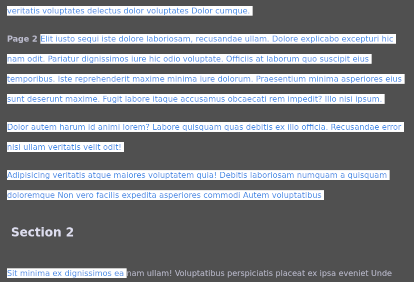
\includegraphics[width=\textwidth]{../src/assets/annotator-documentation/virtual-text.png}
  \end{minipage}%
  \quad%
  \begin{minipage}{9cm}
    \lstset{%
      basicstyle={\scriptsize\ttfamily},
      language=html5,
      showspaces=false,
      showstringspaces=false,
      keywordstyle=\color{blue}\bfseries,
      ndkeywordstyle=\color{green!40!black}\bfseries,
      stringstyle=\color{brown!80!black},
    }
    \begin{lstlisting}
...
<p>
  <strong data-virtual-text="Page 2 "></strong>Elit...
  Dolore explicabo excepturi hic nam odit.
  ...
</p>
...
<h2 data-virtual-text="Section 2"></h2>
<p>
  Sit minima ex dignissimos ea nam ullam!
  ...
</p>
...
    \end{lstlisting}
  \end{minipage}

  \caption{
    (l) Virtual text in a document cannot be selected, and is not part of annotations.
    Virtual text can be placed inline, or as a block element.
    (r) The HTML source code to produce the virtual text above.
  }
  \label{fig:virtual-text}
\end{figure}


In theory, all HTML files should be fine to use for annotation purposes.
However, there might be special considerations to be made about how you want the text to be represented.
In general, I would highly suggest to only use simple, semantic HTML without special styling, images, or even \verb!<script>! tags\footnote{
  While having \texttt{<script>} tags in the HTML of a document is \emph{possible,} I would \textbf{highly discourage} having them.
  Not only might they break the annotator functionality in some way, they open up a major security vulnerability to users of the annotator.
  Before opening up all this functionality to the general public, I intend to add some input sanitation and maybe other security measures to lock this down.
  Adding \texttt{<style>} tags to the HTML should work as intended and may in some cases even be necessary, but I would discourage overusing this.
}.
If you are unsure about any of this, feel free to involve me in the creation of new documents.
Some questions you should think about before creating a HTML document for annotation:

\begin{itemize}
  \item
    Are there sections of the text (e.g., page numbers) that are \emph{\enquote{not really}} part of the text?
    That means: those sections should not be selectable or annotatable.
    Some information on how to incorporate virtual text is given in the paragraph below.
  \item
    Is there text that requires special highlighting or styling?
    Would such styling interfere with the styling of annotated text or the evidence links?
  \item
    Is the text left-to-right (e.g., latin scripts), right-to-left (e.g., Arabic), or even top-to-bottom, right-to-left (e.g., Chinese)?
    Is the writing direction mixed (e.g., English headings in Arabic text)?
\end{itemize}

To add \emph{virtual} text to a document, we use HTML \emph{pseudo-elements,} which are generated by the browser and are not part of the textual content of the document.
Take note that virtual text, therefore, is only possible to add when using HTML, not plain text.
Virtual text has the advantage of being skipped by the offset calculations and not being selected, therefore also not being part of the text selection and the annotation content.
For adding virtual text, add the respective HTML element (e.g., \verb!<h2>! or \verb!<span>!) \emph{without} any text between the tags.
The virtual text itself needs to be passed as an \emph{element attribute} to the text.
The attribute name used is \verb!data-virtual-text!.
The appearance of the virtual text depends on which type of HTML element you use to represent it.
Block-level elements, like headings (\verb!<h1>!, \verb!<h2>!, etc.), will be represented thus, and inline elements, like \verb!<span>!, \verb!<strong>!, or \verb!<em>!, will be placed inline, which might be useful if the virtual text should be within a paragraph (e.g., for sentence numbering).
\cref{fig:virtual-text} shows an example document with two instances of virtual text:
One inline \verb!<strong>! element, and one block-level \verb!<h2>! element.
The HTML content of the document to produce this effect looks as listed in \cref{fig:virtual-text}.


\subsection{Annotations}
\label{sec:annotations}

An \emph{annotation,} in general, consists of a \emph{start} and \emph{end} position within a \emph{document,} as well as an \emph{instance} (see \cref{sec:database-schema} for more details).
Annotations are represented in the text by colored background behind the annotated text passage.
In the following, the user controls of the annotator are described, as well as how to create, edit, and delete annotations.


\subsubsection{The Annotator Interface}
\label{sec:annotation-annotator}

\begin{figure}[htb]
  %

  \caption{
    The annotator consists of of two main components:
    the \emph{document area} on the left, and the \emph{editor pane} on the right.
    A section on the top displays information about the current document.
    Annotations are displayed by colored background behind the annotated text.
    Evidence is represented by links connecting multiple annotations.
    The evidence is ordered into vertical pathways on the left of the document area, so-called \emph{swimlanes.}
  }
  \label{fig:annotator-interface}
\end{figure}

After having selected a document in the document selection screen (\cref{sec:document-selection}), it and its annotations and evidences are displayed in the annotator.
The annotator interface, shown also in \cref{fig:annotator-interface}, consists of two main views.
The \emph{document area} on the left shows the document, annotations, and evidences;
and the \emph{editor pane} on the right shows annotation and evidence editors, when open.

The document area is scrollable, and the document text is displayed here with a large line height to accomodate links between the rows.
A scrollbar on the left of the document area shows the current position in the document, and the positions of annotations are also indicated here.
Annotations within the text are indicated by a colored background, where different colors signify different types of annotations (place, person, religion, time group).

Evidences are groups of one place annotation, one religion annotation, zero or one person annotations, and zero or one time group annotations (see \cref{sec:database-schema}).
In the annotator, they are represented by a line connecting all annotations that are part of the evidence.
If the annotations are in different lines of the text, the line takes a detour via the left margin of the document to avoid crossing text.
In the margin, the evidence links are horizonally distributed into \emph{swimlanes} to avoid overdrawing.
For multiple evidence links going into the same line of text, they are also vertically distributed in the same fashion.

The editor pane is where the annotation or evidence editor is displayed when creating or editing an annotation.
This is described in more detail below.
Initially, the editor pane is empty, as no annotation or evidence is being edited.


\subsubsection{Creating an Annotation}
\label{sec:annotation-creation}

\begin{figure}[htb]
  % 

  \caption{
    Annotation creation starts by selecting a text passage using the mouse.
    Then, a dialog window pops up, where the type of annotation is selected.
    After editing and saving the new annotation, it appears in the text.
  }
  \label{fig:create-annotation}
\end{figure}

The process for creating a new annotation is shown in detail in \cref{fig:create-annotation}.
Initially, the text passage that is to be annotated needs to be selected using \emph{regular text selection;}
that is, going over the start of the text passage with the mouse, push and hold down the left mouse button, drag the mouse until the end of the text passage, and release the left mouse button.
The selection should become highlighted while doing this.

As soon as you release the left mouse button, the selection of the text passage is finished.
The selected text is what will become the annotation.
Because there are four types of annotations, depending on which type of instance is represented (see \cref{sec:database-schema}), next a pop-up window appears, where the type of annotation needs to be selected.
The window also shows the content of the annotation again, and there are four buttons, one for each type of annotation.
By clicking one of the buttons, that type is selected, the pop-up window is closed, and the \emph{annotation editor} is opened.
If you want to re-select the text passage or abort the creation of the annotation for any other reason, you can either click on the red cross in the top right, or anywhere outside of the pop-up window.

Next, in the \emph{editor pane,} an annotation editor appears, where you can fill out the data for that annotation and the connected instance.
This editor window is described in more detail in \cref{sec:annotation-editing}, as the process for creating and editing existing annotations is quite similar.
The only difference is that:

\begin{enumerate}
  \item the button for closing the editor will cancel creation without a prompt,
  \item the delete button at the bottom is instead labeled \emph{\enquote{Cancel creation}} and serves the same function,
  \item the save button at the bottom is instead labeled \emph{\enquote{Create}} and clicking it will persist the new annotation and instance to the database, and
  \item the editor row for changing the text extent of the annotation is missing.
\end{enumerate}

Finally, after clicking \emph{\enquote{Create}} in the editor, the editor will close, and the new annotation will appear in the document.
Annotations \emph{may} overlap, and may even cover exactly the same text passage.
It is completely fine to do a text selection over an existing annotation in the text.
When annotations overlap, the parts where they do are highlighted in gray instead of the normal annotation colors.

\begin{figure}[htb]
  % 
  \caption{
    Suggestions for new annotations are indicated by yellow curly underlining.
    These suggestions are based on known names for entities from the database, as well as existing annotation content.
  }
  \label{fig:annotation-suggestion}
\end{figure}

The server will also generate suggestions for annotations.
These are based on known names (place names, alternative names from other languages, religion and person names) from the database, as well as on existing annotations in the current document.
\cref{fig:annotation-suggestion} shows an example:
The person \emph{Athanasius I bar Gamala} has been annotated in the text previously (under the name \emph{\enquote{Athanasius}}).
Based on that, the suggestion for a person annotation at this position is suggested.
\emph{Clicking} on the annotation suggestion, which is indicated by a yellow curly underline, will open an annotation editor of the respective type, with the suggested entity (place, person, or religion) already selected.
The editor now also indicates where the suggestion stems from.
Clicking \emph{Create} will commit the annotation to the database, replacing the suggestion.


\subsubsection{Selecting an Annotation}
\label{sec:annotation-selection}

\begin{figure}[htb]
  \centering
  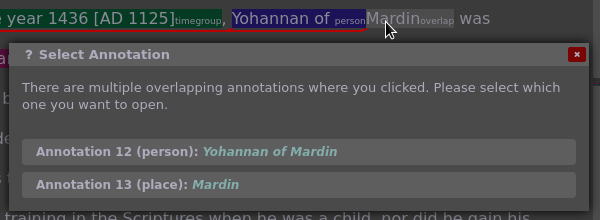
\includegraphics[width=8cm]{../src/assets/annotator-documentation/select-annotation.png}
  \caption{
    When clicking on an overlap between two or more annotations, a pop-up window appears, where you can select which annotation you meant to click on.
  }
  \label{fig:annotation-selection}
\end{figure}

Selecting an annotation is as simple as clicking on it in the document area.
When hovering over the annotation with the mouse, it is already outlined.
Especially in cases where annotations are very long, or there are overlaps with other annotations, this outline can be helpful for understanding which annotation is currently under the mouse cursor.
When annotations overlap and you click on the gray section (i.e., the overlapping part), it is not immediately clear which annotation you want to select.
In that case, a pop-up window appears, listing the different annotation candidates with their type and content (see \cref{fig:annotation-selection}).
By clicking on the intended annotation in the list here, it is selected.
The selection process can be cancelled by clicking on the red cross, or anywhere outside of the pop-up window.


\subsubsection{Editing an Annotation}
\label{sec:annotation-editing}

\begin{figure}[htb]
  \centering
  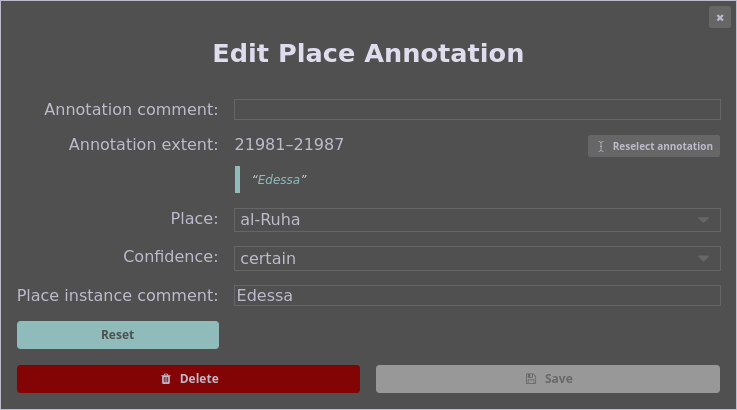
\includegraphics[width=8cm]{../src/assets/annotator-documentation/edit-place-annotation.png}

  \caption{
    The annotation editor for a place annotation.
  }
  \label{fig:edit-place-annotation}
\end{figure}

In the annotation editor, you can edit the \emph{annotation comment,} which is the \verb!comment! field of the record in the \verb!annotation! table.
This might be useful if there is something special about the placement of the annotation in the text, or some useful context.
You can also see and edit the textual extent of the annotation (more details in the next paragraph).
Further, you can edit the \emph{instance} data.
The editors for the different types of annotations, therefore, look slightly different.
\cref{fig:edit-place-annotation} shows an editor for a place annotation:
Here, the annotation comment field is empty.
For the place instance, the place itself, the location confidence, and the comment in the \verb!place_instance! table can be edited.
The place is selected via a drop-down menu, as is the confidence.
The comments are entered using text fields.
For person and religion annotations, the editors look quite similar, but the first drop-down menu lists persons or religions, respectively.

An annotation has a start and end position in the text, which are stored in the \verb!annotation! table of the database.
As the placement of the annotation could need to be changed, the editors provide a way to see the current extent, and to edit it.
Under the title \emph{\enquote{Annotation extent,}} three elements are visible:
A representation of the start and end position of the annotation, a button to start editing, and a text area where the textual content of the annotation is shown.
To change the extent, click on the button, which is initially labeled \emph{\enquote{Reselect annotation}} (see \cref{fig:edit-place-annotation})
The button now turns red and the text says \emph{\enquote{Cancel}} (see \cref{fig:edit-timegroup-annotation}), and clicking it again will go back to the previous state.
By now selecting a text passage in the document area, the textual extent of the annotation will be updated.
As with all other attributes of the annotation and instance, the changes will only be put into the database when clicking on the save button.
The annotation's textual extent can only be edited for existing annotations, and therefore this facility is not displayed when creating a new annotation.

\begin{figure}[htb]
  \centering
  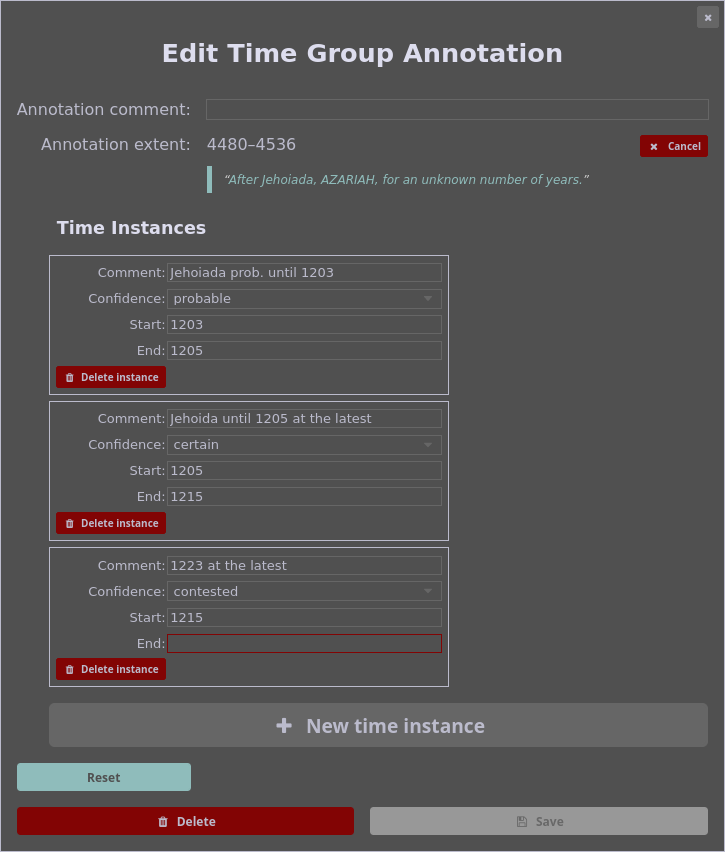
\includegraphics[width=8cm]{../src/assets/annotator-documentation/edit-timegroup-annotation.png}
  \caption{
    The annotation editor for a time group annotation.
    For the third time instance, the mandatory end time field is empty, and the input is therefore outlined in red.
    The user is currently editing the textual extent of the annotation, and the button in that section of the editor therefore reads \emph{\enquote{Cancel.}}
  }
  \label{fig:edit-timegroup-annotation}
\end{figure}

For the time group annotations, the editor looks a bit different because of the way time groups work:
One time group can have zero or more time instances, and all of them would be attributed to the annotation.
\cref{fig:edit-timegroup-annotation} shows an editor for a time group annotation.
Besides the annotation comment and textual extent, time instances are shown as separate items, where the comment, confidence, start time, and end time can be edited.
In this case, start and end time must be numbers, and the end time must be greater than or equal to the start time.
Each time instance can separately be removed by clicking on the \emph{\enquote{Delete instance}} button in the respective box, and new time instances can be added via the large \emph{\enquote{New time instance}} button.
All changes, additions and deletions are only persisted to the database when the entire time group annotation is saved with the save button in the lower right, and are not persisted if the editor is closed, discarding the edits.

Clicking on the \emph{reset} button in the lower left of the editor will revert the values to their initial state, as if the editor was freshly opened.
The editor can be closed by clicking on the cross in the upper right.
If there are unsaved changes, a prompt will appear to confirm that those changes should be discarded.
The green \emph{save} button in the lower right will persist all changes to the database.
The button will be greyed out and disabled if there are no changes to the annotation yet.
The red \emph{delete} button will delete the instance and annotation (see \cref{sec:annotation-deletion}).

All form data in the editor is validated.
If a field is empty \emph{and} mandatory (e.g., no place is selected for a new place annotation), the field will be outlined in red to signify that.
Similarly, if the content of an input field is invalid (e.g., end time before start time for a time instance), it will be outlined in red as well.
In both cases, the save or create button will be disabled and greyed out.


\subsubsection{Deleting an Annotation}
\label{sec:annotation-deletion}

\begin{figure}[htb]
  \centering
  
\includegraphics[width=8cm]{../src/assets/annotator-documentation/delete-annotation.png}

  \caption{
    A confirmation dialog appears when deleting an annotation.
  }
  \label{fig:delete-annotation}
\end{figure}

The red \emph{delete} button in the bottom left of the annotation editor will delete the instance and annotation.
Deleting an instance is only possible if the instance is not part of an evidence, and therefore this button is greyed out and disabled if that is the case.
When clicking on the button, a confirmation dialog will first appear to make sure that this is the intended action, see \cref{fig:delete-annotation}.
When clicking \emph{cancel,} the deletion is not performed.
When clicking \emph{delete,} the annotation and the instance will be removed from the database, and the annotation will disappear from the document area.


\subsection{Evidences}
\label{sec:annotator-evidences}

An \emph{evidence,} in general, is a grouping of a \emph{place instance,} a \emph{religion instance,} and optionally a \emph{person instance} and a \emph{time group} (see \cref{sec:database-schema}).
In addition, the evidence has a comment field, the \emph{interpretation confidence} which specifies how confident you are in the interpretation of the source when creating the evidence, and a visibility flag that controls whether the evidence will appear in the visualization or not.

Each evidence also has a \emph{source instance,} which for annotator-generated evidences is created automatically based on the document's source.
Here, the \emph{source confidence,} which specifies the source's trustworthiness for that specific evidence, can also be set.
Last, evidences can be \emph{tagged} with zero or more tags.


\subsubsection{Selecting an Evidence}
\label{sec:evidence-selection}

\begin{figure}[htb]
  % 

  \caption{
    To select an evidence, hover on the link with the mouse.
    This will already make the link bolder.
    Then clicking the link will select the evidence.
    The link will then turn blue and start to be animated, and the contained annotations are also outlined and animated.
  }
  \label{fig:select-evidence}
\end{figure}

When selecting an evidence, it is opened in the evidence editor.
When creating a new evidence, that new evidence is automatically selected for as long as it is edited.
An existing evidence is selected by clicking anywhere on the link.
The links are layed out in a way that they overlap as little as possible.
To further distinguish which evidence is currently under the cursor, the link gets bolder when the mouse hovers on it.
Clicking on a link will \emph{select} that evidence.
It is then opened in the evidence editor.
Further, the evidence link and the connected annotations are highlighted differently, with blue color and animation, as shown in \cref{fig:select-evidence}.
Selecting a different evidence while the editor is opened will switch to editing that evidence;
however, if there are unsaved changes, a confirmation prompt is shown first.


\subsubsection{Creating an Evidence}
\label{sec:evidence-creation}

\begin{figure}[htb]
  \centering
  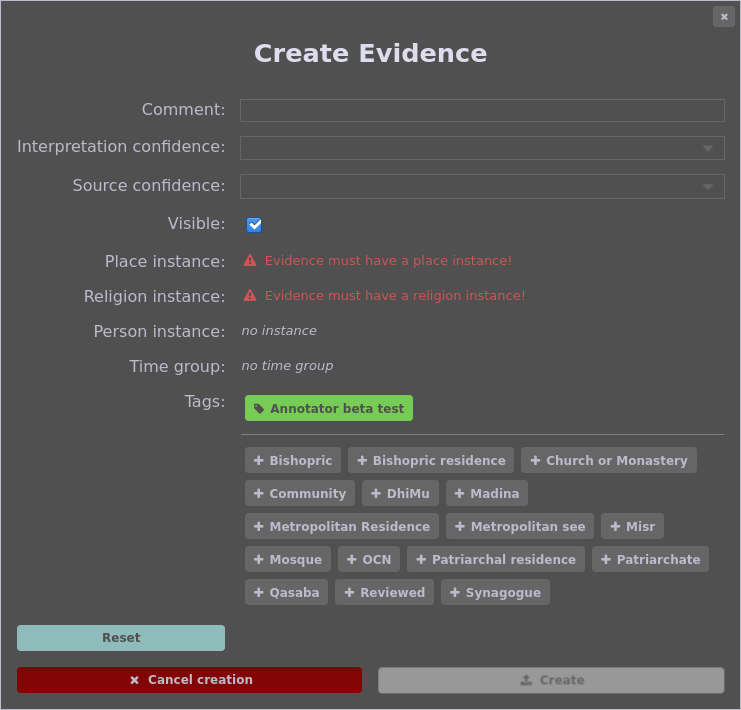
\includegraphics[width=8cm]{../src/assets/annotator-documentation/create-evidence.png}

  \caption{
    Evidence editor for a new evidence.
    The mandatory place and religion instances are empty, and the evidence can therefore not be created yet.
  }
  \label{fig:create-evidence}
\end{figure}

To create an evidence, simply click on the \emph{\enquote{New evidence}} button in the top right of the document area (see \cref{fig:annotator-interface}).
This will open the evidence editor with a new evidence (see \cref{fig:create-evidence}).
While the evidence editor is opened, the button is greyed out and disabled.
As with annotations, creating a new or editing an existing evidence is very similar, and so the description of the editor itself is described below, in \cref{sec:evidence-editing}.
And again, there are slight differences in the three buttons (compare also \cref{fig:create-evidence} and \cref{fig:edit-evidence}).

\begin{enumerate}
  \item the button for closing the editor will cancel creation without a prompt,
  \item the delete button at the bottom is instead labeled \emph{\enquote{Cancel creation}} and serves the same function, and
  \item the save button at the bottom is instead labeled \emph{\enquote{Create}} and clicking it will persist the new evidence to the database.
\end{enumerate}


\subsubsection{Editing an Evidence}
\label{sec:evidence-editing}

\begin{figure}[htb]
  \centering
  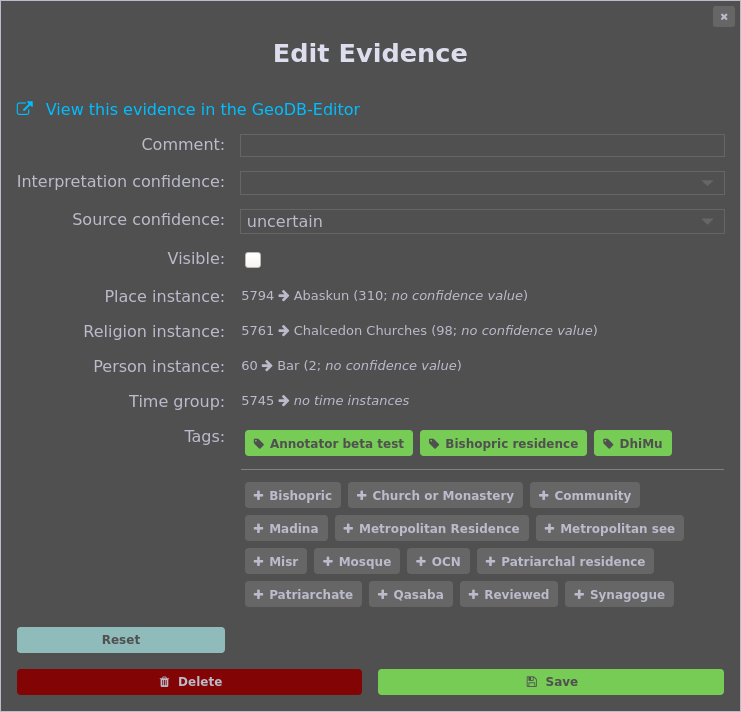
\includegraphics[width=8cm]{../src/assets/annotator-documentation/edit-evidence.png}

  \caption{Evidence editor for an existing evidence.}
  \label{fig:edit-evidence}
\end{figure}

The evidence editor, shown in \cref{fig:create-evidence} and \cref{fig:edit-evidence}, contains four traditional form fields, which are all optional.
These form fields can be edited in a straightforward manner:

\begin{itemize}
  \item a text field for the \verb!comment! field of the evidence,
  \item a drop-down menu for the evidence's \emph{interpretation confidence,}
  \item a drop-down menu for the source instance's \emph{source confidence,} and
  \item a checkbox to toggle the visibility of the evidence in the visualization\footnote{
      Evidence tuples that do not have the \texttt{visible} flag set are \emph{never loaded} from the database.
      While most other filters in the visualization will hide or show evidence dynamically, evidences that are not \emph{visible} will never show up.
      Of course, the visibility can be changed later.
    }.
\end{itemize}

\begin{figure}[htb]
  % 

  \caption{
    To toggle membership of an annotation, and its associated \emph{instance,} to an evidence, click on the annotation while the evidence editor is opened.
    The link representing the evidence will update instantly.
  }
  \label{fig:edit-evidence-membership}
\end{figure}

The next four rows represent the place instance, religion instance, person instance, and time group that are part of the evidence.
Here, as the place and religion instance are mandatory, these will show up as red when empty (see \cref{fig:create-evidence}).
These four fields cannot be directly edited (i.e., by clicking or typing in them), but instead are controlled via the \emph{document area.}
While the editor is opened, the annotations that are part of the evidence are outlined in blue and animated.
Changing membership of annotations works as follows (see also \cref{fig:edit-evidence-membership}):
To add an annotation and its instance to the evidence, \emph{click} on the annotation.
To remove an annotation and its instance that are already part of the evidence, also \emph{click} on the annotation (clicking \emph{toggles} membership).
If the evidence already contains an instance and annotation of a certain type, clicking on a \emph{different} annotation of that type \emph{replaces} the previous instance and annotation with the new ones;
for example, if there are two place annotations in the text, one for \textbf{Edessa} and one for \textbf{Damascus,} with \textbf{Edessa} being part of the evidence, clicking on the \textbf{Damascus} annotation would replace the place instance in the evidence, and the evidence would now be related to the place Damascus.
An instance and annotation can be associated with multiple evidences.

The fields in the editor displaying the instances cannot be interacted with directly.
They show more information on the instances themselves and update automatically.
In particular, they show the instance ID, the name and ID of the entity the instance refers to (place, religion, or person), and the respective instance confidence.
For the time group, a comma-separated list of all time instances, with start time, end time, and confidence is shown instead.
The data about the instances must be fetched from the database when it changes, so directly after opening the editor, or when toggling membership of an annotation and instance, the data is not available for a short while, and a loading indicator is shown instead.

If no instance of that type is connected, this is indicated instead, as shown in \cref{fig:create-evidence}.
As the place and religion instances are mandatory, the absence of those is highlighted in red with more urgency.

The last part of the evidence editor is the evidence tags.
Evidence can be tagged to create specific groups of evidences;
for example, evidences that refer to Bishopric residences, or evidences that have been thoroughly reviewed.
An evidence can have zero or more tags.
For now, all evidence created via the annotator will have the tag \emph{Annotator beta test} assigned to them, and the tag cannot\footnote{
  The tag cannot be removed using the annotator.
  However, it is possible to remove it from the evidence via the GeoDB-Editor.
  Only do this if you are certain you want to remove the association!
} be removed.
The idea is that, until we are sure the annotator does not do anything harmful to the database, we will be able to identify and remove all evidence that was added to the database via the annotator if we so choose.
Of course, we can always remove the tag from the evidences later.
Tags that are associated with the evidence are displayed at the top in green, tags that are not are displayed below in grey, with a \emph{plus} symbol instead of the \emph{tag} symbol.
To remove an associated tag, click on it, and it moves to the bottom.
Similarly, to add a tag, click on it, and it moves up and becomes green.

As with the annotation editor, all changes made are only local until you click the \emph{save} button at the bottom (or, for new evidences, the \emph{create} button).
Using the \emph{reset} button, the initial state from the database can be restored for all fields, discarding all changes.
Clicking on the cross in the top right closes the editor if there are no unsaved changes, otherwise a confirmation prompt is shown first.
The same prompt is also shown when trying to open a different evidence by clicking on the respective link in the document area.
The \emph{delete} button deletes the evidence, see \cref{sec:evidence-deletion}.
The \emph{save} button will persist all changes to the database.
This button will only be enabled if it is currently possible to save:
If there are no changes, it is disabled and greyed out.
Further, if there is invalid input (i.e., no place or religion instance selected), saving is also not possible.

For evidence that is already saved in the database (i.e., when editing evidence, but not during creation), the evidence editor also shows a link at the top labeled \emph{\enquote{View this evidence in the GeoDB-Editor.}}
Clicking this link will open the GeoDB-Editor, and there select the place of the evidence, scroll down to the evidence table, and select the evidence there as well.
For evidence created using the annotator, a similar link exists in the evidence table of the GeoDB-Editor, which opens the appropriate document in the annotator and opens the respective evidence in the evidence editor.


\subsubsection{Deleting an Evidence}
\label{sec:evidence-deletion}

\begin{figure}[htb]
  \centering
  
\includegraphics[width=8cm]{../src/assets/annotator-documentation/delete-evidence.png}

  \caption{A confirmation dialog appears when deleting an evidence.}
  \label{fig:delete-evidence}
\end{figure}

Clicking on the red \emph{delete} button in the evidence editor will delete the evidence from the database.
A confirmation dialog (see \cref{fig:delete-evidence}) will appear first to avoid accidental deletions.
In the case of new evidences that have not been saved yet, the button will instead be labeled \emph{\enquote{Cancel creation.}}

Deleting an evidence will \emph{not} delete the connected annotations and instances.
Those will remain in the database and the document area.
It will only delete the evidence itself, the source instance, and all tag associations.
The deletion will be reflected at once in the document area, where the respective link will also disappear.
After deletion, the evidence editor is closed.


\section{Place URI List}


\section{Reporting}
\label{sec:reporting}


\section{Other Pages}


\subsection{Documents}

The documents page contains links to a few smaller pages and utilities.
Some of these are not available to all users, but only to developers or administrators.
Besides the page links listed in the following, the documents page also has links to the report creation page and the list of existing reports detailed in \cref{sec:reporting}.

\paragraph*{Database edit log.}
This page is visible only to administrators (role \verb!admin!).
It details the contents of the \verb!user_action! table in reverse chronological format.
This data can be reviewed for provenance, or to quickly retrieve an old value from a database entry after a mistake in an edit.

\paragraph*{REST API documentation.}
This page is visible to all developers (role \verb!dev!), and contains a list of the endpoints in the REST API (see~\cref{sec:rest-api}).
They are the HTTP endpoints under \verb!/rest/!, which are listed in the form they are defined in Flask.
The URL and possible HTTP verbs are extracted from Flask runtime information, and the documentation string is taken directly from the Python \emph{docstring} of that method.
The REST API methods' docstring are all quite detailed and show request and response content types, possible values and data entries, and payload or response examples, where applicable.

\paragraph*{Annotator user guide.}
The annotator user guide explains how the annotator works and is used in great detail, and with example images.
This page is visible to all users with the \verb!annotator! role.
The annotator user guide is the basis for the text in \cref{sec:annotator}.

\paragraph*{PostgreSQL Database Schema.}
Download link to a PDF of the database structure.
This link is available to all developers (role \verb!dev!) and to users with the \verb!pgadmin! role.
The PDF is the same as \cref{fig:db-structure}, enclosed in a page with headers and footers.

\paragraph*{Download database dump.}
Download link to a SQL dump of the entire database.
The file is served as GZIP-ed SQL, and is generated on the fly.
This functionality is available to all users.
However, if the requesting user does \emph{not} have the \verb!admin! role, the dump is data-only, and also omits the \verb!action_type!, \verb!user!, and \verb!user_action! provenance tables described in \cref{sec:provenance-tables}.


\subsection{GDPR, Imprint, Cookie Preferences}

A separate blueprint serves pages for the GDPR\footnote{
  \textbf{GDPR:} General Data Protection Regulation of the European Union.
  Called DSGVO \emph{(Datenschutzgrundverordnung)} in German.
}
content.
These pages are accessible even without login, and are available as links in the footer of each page\footnote{
  In the visualization, which has a tighter layout without a footer, these links are placed in the header instead.
}.
A general data protection page states what data is collected from visitors, and what rights they have under GDPR.
The imprint \emph{(Impressum)} page contains information about how to get in touch with the website administrators.
Finally, the websites use cookies and \verb!localStorage! to store state and information on the user's computer.
These are used for login, but also for functionalities such as storing table or visualization layout.
In accordance to \S\,7 \P\,2 GDPR, consent to store these cookies needs to be given explicitly by users.
For this, they are shown a consent popup when they first visit the site, with the choices of
\begin{enumerate*}[label=(\arabic*)]
  \item no cookies,
  \item only necessary cookies, or
  \item all cookies.
\end{enumerate*}
Users must be able to amend or withdraw consent at any time (\S\,7 \P\,3 GDPR), so the consent settings shown in the popup are also available as a separate page.

Users must consent to necessary cookies (option (2)) to be able to login, as the session cookie must be stored.
Further, the consent itself is stored as a cookie.
Consequently, visitors who reject all cookies (option (1)) will be shown the cookie consent popup each time they open a page, as there is no way to store their choice.
The \enquote{all cookies} option (3) is necessary to use additional features such as storing custom visualization and table layouts.

When hosting the Damast system somewhere else, a different imprint than the default one is needed if the administrators and hosting organization differ.
Probably, the data protection page needs to be modified as well.
Here, the blueprint override functionality discussed in \cref{sec:override-blueprints} can come in handy.


\subsection{Login and Password Management}

A blueprint provides login and logout functionality, as well as a page to change the current user's password.
These are linked in the top right of the page, in the header.
If a visitor is not logged in, a link to the login page is shown there.
If they are logged in, the user's name, a link to the password change page and a link to log out is shown.

On the password change page, the user must enter their current and their new password, and then submit.
The server backend will check that the old password matches, and that the new password has sufficient complexity (entropy).
If that is the case, the password hash is updated in the user database and the session token is renewed.


\printbibliography

\end{document}
